\documentclass[12pt]{article}

% Paquetes comunes
\usepackage[utf8]{inputenc}     % Codificación
\usepackage[T1]{fontenc}        % Fuente
\usepackage[english]{babel}     % Idioma
\usepackage{amsmath, amssymb}   % Matemáticas
\usepackage{graphicx}           % Imágenes
\usepackage{float}              % Posición de figuras
%\usepackage{cite}               % Citas
\usepackage{hyperref}           % Enlaces
\usepackage{geometry}           % Márgenes
\geometry{a4paper, margin=2.5cm}
\usepackage{color}              % Colores 
%\usepackage{qrcode}             % Código QR  

\usepackage{csquotes}
%\usepackage[style=numeric,sorting=none]{biblatex}

\usepackage[backend=biber,style=numeric,sorting=none]{biblatex}
\addbibresource{refs.bib}  

\usepackage[inline]{enumitem} % Paquete necesario para listas en línea
\setlist[enumerate,1]{label=(\roman*)} % Estilo de la etiqueta: (i), (ii), 

\usepackage{booktabs} % Para tablas
\usepackage{tabularx}
\usepackage{threeparttable}
\usepackage{multirow}
\usepackage{makecell}

\usepackage{pgfplots}
\usetikzlibrary{matrix}
\pgfplotsset{compat=1.18}



\title{Detection of Vascular Pathologies in Non-Contrast Magnetic Resonance Images for Early Screening} %of Cerebrovascular Diseases}
\author{Patricia García-Berlanga, Juan F. Zapata-Pérez, \\ 
        Pablo Casado Martínez, \\ 
        Juan de la Cruz Mártinez Cabeza de Vaca-Alajarín}
\date{\today}

\begin{document}

\maketitle

% Original abstract kept commented for context (minor edits allowed in comments)
%\abstract{
%Cerebrovascular diseases (CVD) are a leading cause of death and disability worldwide. Early detection and treatment are crucial to prevent severe outcomes. Magnetic Resonance Imaging (MRI) is a powerful tool for diagnosing CVD, but the use of contrast agents can pose risks to patients. This study aims to develop a method for detecting vascular pathologies in non-contrast MRI images, enabling early screening of CVD. We propose a deep learning-based approach that leverages convolutional neural networks (CNNs) to analyze non-contrast MRI scans and identify vascular abnormalities. The model is trained on a dataset of annotated MRI images, and its performance is evaluated using metrics such as accuracy, sensitivity, and specificity. Preliminary results indicate that the proposed method can effectively detect vascular pathologies, with potential applications in clinical settings for early CVD screening. Further research will focus on refining the model and validating its performance on larger datasets.
%
%Accurate segmentation of ischemic stroke lesions in magnetic resonance imaging (MRI) is essential for early diagnosis and treatment planning. This study evaluates and compares the performance of three deep learning architectures—U-Net, nnU-Net, and YOLOv8—for the automatic segmentation of ischemic stroke lesions using FLAIR MRI sequences without contrast agents. The models were trained and tested on the ISLES 2022 public dataset, containing 250 patient cases. U-Net was manually configured as a 3D baseline model, nnU-Net was applied as a self-configuring 3D full-resolution mode, and YOLOv8 was adapted from object detection to 2D medical image segmentation. Performance was assessed using the Dice coefficient and Intersection over Union (IoU) metrics. Results show that nnU-Net achieved the best overall accuracy, with a mean Dice score of 0.483 ± 0.284, outperforming both U-Net and YOLOv8. YOLOv8 demonstrated the fastest inference and competitive segmentation accuracy, indicating potential for real-time clinical use. U-Net exhibited limited generalization across heterogeneous lesions. In conclusion, nnU-Net remains the most reliable and adaptive solution for MRI stroke lesion segmentation, whereas YOLOv8 offers a promising lightweight alternative for time-critical applications. These findings highlight that automated segmentation of ischemic lesions from non-contrast FLAIR MRI is feasible and may support faster, more objective, and clinically scalable stroke assessment.
%
%resumen de lo anterior. Abstract, adaptado a este trabajo:
%
%Cerebrovascular diseases (CVD) are a leading cause of death and disability worldwide, making early detection and treatment crucial to prevent severe outcomes. This study addresses the clinical need for non-contrast MRI-based detection methods by developing a deep learning approach to identify vascular pathologies and segment ischemic stroke lesions without contrast agents. We evaluated and compared three convolutional neural network architectures—U-Net, nnU-Net, and YOLOv8—for automatic segmentation of ischemic stroke lesions using FLAIR MRI sequences. The models were trained and tested on the ISLES 2022 public dataset containing 250 patient cases. Performance was assessed using Dice coefficient and Intersection over Union (IoU) metrics. Results demonstrate that nnU-Net achieved the best overall accuracy with a mean Dice score of 0.483 ± 0.284, outperforming both U-Net and YOLOv8 in reliability and generalization across heterogeneous lesions. Conversely, YOLOv8 demonstrated the fastest inference speed and competitive segmentation accuracy, positioning it as a promising lightweight alternative for time-critical clinical applications. These findings confirm that automated segmentation of ischemic lesions from non-contrast FLAIR MRI is feasible and clinically viable, supporting faster, more objective, and scalable stroke assessment in clinical settings. Further research will focus on validating these models on larger datasets and refining their performance for enhanced early CVD screening capabilities.
%
%}

\abstract{
Early and non-invasive detection of cerebrovascular pathologies is essential to improve patient triage and outcomes. Contrast-free FLAIR MRI sequences are widely available in clinical practice but pose challenges for automated analysis due to variable lesion appearance, low contrast, and inter-scanner variability. In this study, we evaluate and compare three deep learning strategies for ischemic lesion segmentation in non-contrast FLAIR images: a classical 3D U-Net, the self-configuring nnU-Net framework, and an adapted 2D YOLOv8 segmentation variant. All methods were trained and tested using the ISLES 2022 dataset (N = 250 cases) under matched preprocessing and evaluation protocols to ensure a fair comparison.
%
We report quantitative performance using Dice similarity coefficient and Intersection over Union (IoU), and analyze trade-offs between accuracy, robustness and inference efficiency. The nnU-Net achieved the highest average overlap (Dice $= 0.483 \pm 0.284$), demonstrating superior robustness across heterogeneous lesion presentations. The YOLOv8-based model provided competitive volumetric performance (Dice $\approx 0.476$) while substantially reducing inference time, suggesting suitability for time-constrained clinical workflows. The classical 3D U-Net served as a manual baseline and exhibited lower mean overlap (Dice $\approx 0.294$), indicating sensitivity to parameter tuning and dataset variability.
%
Beyond numerical metrics, we qualitatively examine typical failure modes (small peripheral lesions, diffuse low-contrast areas and spatial mismatches between masks and images) and discuss preprocessing steps that mitigate them (spatial resampling, intensity normalization, and patch-based training). Finally, we outline practical recommendations for deploying automated segmentation in clinical settings: favor self-configuring frameworks like nnU-Net when compute resources permit, consider lightweight 2D models such as YOLOv8 for fast screening, and ensure rigorous cross-site validation before clinical use.
}

%\tableofcontents
%\newpage


\section{Introduction} \label{sec:introduction}

% Original Introduction preserved below for reference (commented):
% Ischemic stroke is one of the leading causes of disability and mortality worldwide, representing a major challenge for healthcare systems, with significant clinical and economic implications. A rapid and accurate diagnosis is crucial to initiate the appropriate treatment and to reduce long-term neurological deficits in patients\footnote {\url{https://medlineplus.gov/spanish/ency/article/000726.htm}}. In this context, medical imaging plays an essential role in the detection and delineation of brain regions affected by stroke. This process of identifying and outlining the affected regions is commonly referred to as image segmentation, a central task in medical image analysis.  Among the different imaging modalities, magnetic resonance imaging (MRI) stands out as a key tool thanks to its ability to provide detailed anatomical and functional information without exposing patients to ionizing radiation.
% 
% The segmentation of ischemic lesions in MRI scans is a particularly demanding task. Traditionally, this process has relied on manual annotations by radiologists and other clinical experts. Although this approach is precise, it is also labor-intensive, time-consuming, and prone to inter-observer variability. These limitations hinder its applicability in large-scale clinical settings and delay the diagnosis of patients in acute or subacute stages. For this reason, the automation of lesion segmentation has been a long-standing goal in medical image analysis.
% 
% Classical image processing methods, including thresholding, region growing, clustering, and deformable models, have historically been applied in medical image segmentation. While these techniques can provide valuable insights, their performance is specially hindered by inherent challenges in medical imaging, such as anatomical variability among patients, low tissue contrast, imaging artifacts, and the high similarity between healthy and pathological regions. These limitations frequently result in inconsistent or suboptimal segmentation outcomes. Machine learning approaches, particularly support vector machines and random forests, represented a step forward by leveraging handcrafted features. However, these methods still rely heavily on feature engineering, which restricts their adaptability and generalization to new datasets.
% 
% In recent years, deep learning (DL) has revolutionized the field of medical image analysis by overcoming many of the limitations of traditional techniques \cite{Liu2021}. Convolutional neural networks (CNNs) and their derivatives enable the automatic extraction of hierarchical features directly from raw image data, removing the need for manual feature design and significantly improving segmentation performance. Architectures such as U-Net and its variants have become the gold standard for biomedical image segmentation, demonstrating remarkable accuracy and robustness across multiple clinical applications. Moreover, DL-based methods provide consistency across many patients and can accelerate clinical workflows by reducing the burden on radiologists.
% 
% Despite these advances, the application of DL in ischemic stroke segmentation remains a complex challenge. Stroke lesions often exhibit heterogeneous appearances across patients, making them difficult to capture with a single segmentation strategy. Furthermore, the scarcity of annotated medical data adds an additional layer of difficulty. In this scenario, comparing different state-of-the-art architectures provides valuable insights into their strengths and weaknesses, as well as their potential for translation into real-world clinical environments.
% 
% The present research specifically focuses on the automatic segmentation of ischemic stroke lesions in FLAIR MRI sequences without the use of contrast agents. This choice is clinically relevant, as FLAIR images highlight hyperintense regions corresponding to edema and infarcted tissue, while avoiding the risks associated with contrast administration. The study explores and compares three distinct deep learning architectures:\begin{enumerate*}[label=(\roman*)]
% \item U-Net: A widely adopted architecture known for its encoder-decoder structure and skip connections, which facilitate the capture of both local and global context in images.
% \item nnU-Net: An advanced, self-configuring framework that automatically adapts its architecture and training protocols to the specific characteristics of the dataset, often achieving state-of-the-art results with minimal manual intervention.
% \item YOLOv8: A recent evolution of the YOLO family, originally designed for real-time object detection. This architecture is adapted here for 2D medical image segmentation, offering a lightweight and efficient alternative.
% \end{enumerate*}
% 
% The models are trained and evaluated using the ISLES 2022 public dataset \cite{inproceedings}, which includes a diverse set of 250 patient cases with expert-annotated ischemic lesions. The performance of each architecture is assessed using standard metrics such as the Dice coefficient and Intersection over Union (IoU), providing a comprehensive evaluation of their segmentation capabilities.
% 
% The specific objectives of this research are:\begin{enumerate*}[label=(\roman*)]
%   \item To implement and train U-Net, nnU-Net, and YOLOv8 architectures on a public dataset of ischemic stroke MRI scans.
%   \item To evaluate and compare their performance using standard segmentation metrics, including the Dice coefficient and Intersection over Union (IoU).
%   \item To analyze the strengths and limitations of each model in order to assess their potential clinical applicability.
% \end{enumerate*}
% 
% The remainder of this article is structured as follows. Section 3 reviews the state of the art in medical image segmentation, focusing on both classical and deep learning approaches. Section 4 describes the dataset, preprocessing steps, and methodological details of the implemented models. Section 5 presents the experimental results, followed by a discussion in Section 6 that highlights the comparative analysis, limitations, and future directions. Finally, Section 7 summarizes the main conclusions.

% Polished Introduction (biomedical, larger paragraphs):
Ischemic stroke remains a leading cause of death and long-term disability worldwide, imposing substantial clinical and economic burdens on healthcare systems. Rapid and accurate identification of ischemic lesions is critical to guide acute management and rehabilitation planning. In routine clinical practice, Fluid-Attenuated Inversion Recovery (FLAIR) MRI is frequently acquired because it enhances conspicuity of edema and chronic infarcts without the need for intravenous contrast, but FLAIR images present considerable challenges for automated interpretation: lesions can be small, heterogeneous in intensity and shape, and their appearance is often confounded by age-related white matter hyperintensities, motion artifacts and scanner-dependent variations. These factors limit the performance of traditional intensity-based and handcrafted-feature methods and motivate the application of data-driven algorithms capable of learning robust, hierarchical representations directly from imaging data.

Recent advances in deep learning (DL), particularly convolutional neural networks (CNNs), have produced state-of-the-art results in medical image segmentation across multiple anatomies and modalities \cite{Liu2021,ronnebergerUNetConvolutionalNetworks2015}. Architectures such as U-Net and its 3D extensions have become standard baselines, while frameworks like nnU-Net have demonstrated that automated protocol selection and self-configuration often outperform manually tuned pipelines on heterogeneous biomedical datasets \cite{Isensee2021}. At the same time, light-weight, real-time capable architectures originally developed for natural images (for example the YOLO family) have been adapted for segmentation tasks, offering favourable inference speed that can be important in time-critical clinical workflows. However, direct comparisons between fundamentally different paradigms—manual 3D models, self-configuring medical frameworks, and adapted 2D real-time models—remain limited for ischemic stroke segmentation on non-contrast FLAIR data.

This study addresses this gap by conducting a systematic and reproducible comparison of three representative strategies: a manually configured 3D U-Net, the self-adapting nnU-Net framework, and a YOLOv8-based segmentation variant adapted to slice-wise FLAIR inputs. We use the ISLES 2022 public dataset (N = 250) to ensure a standardized benchmark and apply identical preprocessing steps (spatial resampling, intensity normalization and mask alignment), matching evaluation metrics and data splits to minimize sources of bias. Beyond reporting Dice and IoU scores, we analyze robustness across lesion sizes and types, characterize typical failure modes (e.g., missed peripheral lesions, over-segmentation in regions with white-matter hyperintensities), and measure inference efficiency to provide practical trade-offs relevant for clinical deployment.

Our contributions are threefold: (i) a controlled empirical comparison of three distinct segmentation paradigms on non-contrast FLAIR stroke data; (ii) a detailed analysis of preprocessing and training choices that materially affect performance and generalization; and (iii) pragmatic recommendations for integrating automated segmentation into clinical or research workflows, balancing accuracy, robustness and computational cost.

Magnetic Resonance Imaging (MRI) occupies a central role in the diagnosis and management of cerebrovascular disease because it provides high soft-tissue contrast and multiple pulse sequences that highlight different pathophysiological aspects of ischemia (e.g., diffusion restriction on DWI, edema on FLAIR, and perfusion changes on PWI). In many clinical contexts, rapid assessment of MRI—often in conjunction with CT—determines eligibility for reperfusion therapies and guides early care decisions. FLAIR sequences are particularly useful for visualizing subacute and chronic ischemic lesions and are widely available across scanners and centers, making them attractive inputs for large-scale automated analysis pipelines. However, MRI interpretation requires expert neuroradiological training and is subject to inter-reader variability, especially in borderline or small-volume lesions. Automated segmentation systems can therefore augment clinical workflows by providing consistent, reproducible lesion delineations, quantitative volume estimates, and candidate regions for focused radiologist review, potentially reducing time-to-report in acute settings and improving case triage in high-volume clinics \cite{Litjens2017,Esteva2021}.

Deep learning methods offer a practical route to learn complex and hierarchical representations of medical images directly from data, enabling improved sensitivity to subtle lesion features and greater robustness to image variability compared with handcrafted pipelines \cite{Liu2021,Isensee2021}. When carefully validated, these models can operate as decision-support tools rather than replacing clinical judgment: they can flag suspicious regions, provide uncertainty estimates or confidence maps, and accelerate repetitive tasks such as volumetric quantification. Critical considerations for clinical translation include cross-site generalization, interpretability of model outputs, computational requirements for deployment (real-time vs. batch processing), and integration with existing radiology infrastructure (PACS, reporting systems). In this work, in addition to evaluating segmentation accuracy, we measure inference speed and analyze failure cases to inform realistic deployment scenarios and the design of human–AI workflows that preserve clinician oversight and patient safety.

The remainder of the manuscript details related work (Section \ref{sec:relatedwork}), describes dataset preparation and model implementations (Section \ref{sec:methodology}), presents quantitative and qualitative results (Section \ref{sec:results}), and discusses limitations and future directions before concluding.

\section{Related Work} \label{sec:relatedwork}

Medical image segmentation has been a focal point of research for several decades, with significant advancements driven by both classical image processing techniques and the more recent adoption of deep learning methodologies. This section provides an overview of the key developments in this field, highlighting the evolution from traditional methods to state-of-the-art deep learning architectures.

\subsection{Scientific and Technical Context} \label{subsec:context}

While the clinical motivation for ischemic stroke lesion segmentation has been outlined in Section 1, it is equally important to situate this problem within the broader technical landscape of medical image analysis. Stroke lesion segmentation is among the most difficult challenges in brain imaging because of several specific characteristics: (i) lesions exhibit high inter-patient variability in size, shape, and location; (ii) tissue contrast in relevant MRI sequences such as FLAIR is often low, making lesions difficult to distinguish from surrounding white matter; (iii) infarcts evolve over time, so the appearance of acute, subacute, and chronic lesions differs substantially; and (iv) motion artifacts and scanner-dependent variations further complicate analysis. These aspects make the problem more complex than other established tasks such as brain tumor segmentation or multiple sclerosis lesion detection.

A major driver of technical progress has been the creation of benchmark challenges, in particular the ISLES series (Ischemic Stroke Lesion Segmentation) organized within the MICCAI community. These challenges have provided publicly available datasets, standardized evaluation metrics, and competitive leaderboards, enabling direct comparison across methods. Through ISLES, researchers have repeatedly confirmed that conventional intensity-based methods struggle, while data-driven and deep learning techniques consistently achieve superior performance. 

\subsection{Classification of Existing Approaches} \label{subsec:classification}

Segmentation strategies for stroke imaging can be categorized into three major groups: traditional image processing methods, classical machine learning, and modern deep learning-based approaches.

Traditional image processing methods were the first to be applied to medical image segmentation. Thresholding techniques assign pixels to foreground or background based on intensity values, but they fail when tissue contrast is low. Region growing methods start from a seed point and iteratively aggregate neighboring pixels with similar intensity; however, they are sensitive to noise and initialization. Clustering approaches, such as k-means, group voxels according to statistical similarity, but lack spatial constraints and often oversegment complex structures. For instance, K-means has been applied in stroke lesion segmentation to identify hyperintense regions in brain images \cite{inproceedings}, demonstrating moderate success when combined with fuzzy clustering. Deformable models, including active contours (snakes) and level sets, introduce shape priors and regularization, allowing more flexible adaptation to object boundaries. Active contour models have been successfully applied in medical image segmentation, including brain scans, to delineate ischemic stroke lesions \cite{qianActiveContourModel2013}. Similarly, statistical and deformable model approaches have been explored specifically for MRI-based ischemic stroke segmentation, highlighting their potential and limitations in handling heterogeneous lesion shapes \cite{steinStatisticalDeformableModel2001}. Although these methods represented an advance over purely intensity-based techniques and provided valuable insights in early neuroimaging studies, they remain prone to convergence issues, require careful parameter tuning, and are rarely competitive against modern learning-based approaches.

Classical machine learning methods brought the use of data-driven classifiers trained on handcrafted features. Typical features included intensity histograms, texture descriptors, local gradients, or wavelet coefficients. Support vector machines (SVMs), random forests, and shallow neural networks were widely applied. For example, Geremia et al. \cite{geremiaSpatialDecisionForests2011} demonstrated the potential of random forests for lesion segmentation in multiple sclerosis, showing improved generalization compared to thresholding. In the context of ischemic stroke, random forests and SVMs have been applied to diffusion-weighted and FLAIR MRI to segment infarcted regions, achieving moderate accuracy \cite{inproceedings}. These studies highlight that while classical machine learning approaches can improve segmentation over simple intensity-based methods, their performance is limited by the quality and representativeness of handcrafted features. Another limitation is that feature extraction pipelines are often dataset-specific, reducing transferability to new data. In addition, these models do not scale well to high-dimensional medical imaging datasets compared to modern deep learning approaches.

Deep learning methods have redefined the state of the art in medical image segmentation. Convolutional neural networks (CNNs) automatically learn hierarchical representations of the data, reducing the need for manual feature engineering. Fully convolutional networks (FCNs) introduced end-to-end learning for dense predictions. The U-Net architecture \cite{ronnebergerUNetConvolutionalNetworks2015} became a landmark in biomedical image segmentation, with its encoder-decoder structure and skip connections enabling high-level contextual feature extraction and fine spatial localization, particularly relevant for small ischemic infarcts. Variants such as residual U-Nets, attention U-Nets \cite{oktayAttentionUNetLearning2018}, and multi-scale 3D U-Nets \cite{kamnitsasEfficientMultiscale3D2017} have demonstrated improved performance by incorporating residual connections, attention mechanisms, and multi-modal MRI inputs (e.g., DWI and FLAIR) for stroke lesion segmentation.

Frameworks like nnU-Net \cite{isenseeAbstractNnUNetSelfadapting2019} propose a fully automated strategy, self-configuring network depth, patch size, preprocessing, and training parameters to achieve robust performance across multiple medical imaging tasks, including ischemic stroke. Beyond U-Net derivatives, ensembles of fully convolutional networks have been applied to stroke and white matter hyperintensity segmentation, showing enhanced robustness and accuracy \cite{liFullyConvolutionalNetwork2018}.

Other deep learning architectures originally developed for volumetric or general segmentation have also been adapted to medical imaging. Examples include DeepMedic \cite{kamnitsasEfficientMultiscale3D2017} for multi-scale 3D CNNs with probabilistic inference, V-Net for volumetric segmentation, and 2D CNN-based frameworks for ischemic stroke lesion segmentation \cite{shah2DCNNBasedSegmentation2020,gheibiCNNResDeepLearning2023}. Additionally, general-purpose segmentation models such as SegNet and DeepLabv3+, initially designed for natural images, have been successfully applied to medical imaging tasks including stroke and brain lesion segmentation.

More recently, YOLO-based models have been explored for ischemic stroke lesion detection and segmentation, leveraging their speed and efficiency for real-time clinical applications. For example, MSA-YOLOv5 \cite{chenMSAYOLOv5MultiscaleAttentionbased2023} incorporates multi-scale attention mechanisms to improve detection of small and low-contrast lesions in multimodal MRI images. Similarly, lightweight models such as TE-YOLOv5 \cite{chenAutomaticDetectionStroke2022} have demonstrated effective segmentation of diffusion-weighted imaging (DWI) stroke lesions while reducing computational requirements. These studies illustrate the potential of YOLO architectures to complement traditional 3D CNNs, offering rapid inference and promising accuracy, particularly in scenarios where real-time performance is critical.

These deep learning methods outperform traditional and classical machine learning approaches, especially in handling high-dimensional data and complex lesion variability. Nevertheless, they require large annotated datasets, substantial computational resources, and careful design choices or automated configuration strategies to generalize effectively across patients and imaging modalities.

\subsection{Knowledge Gaps and Our Contribution} \label{subsec:gaps}

Several knowledge gaps remain in the current state of the art. First, there is a scarcity of large annotated ischemic stroke datasets, especially for FLAIR sequences, which limits the potential of deep learning models. Second, while U-Net and nnU-Net are widely studied, the applicability of emerging general-purpose segmentation models like YOLOv8 in the biomedical domain remains underexplored. Third, few systematic comparative studies have been conducted across models with fundamentally different design philosophies: U-Net as a domain-specific baseline, nnU-Net as a self-configuring medical framework, and YOLOv8 as a general-purpose real-time model.

The present study addresses these gaps by conducting a comparative analysis of U-Net, nnU-Net, and YOLOv8 for ischemic stroke lesion segmentation using FLAIR MRI. Although trained on a relatively small dataset, the results indicate that these models can achieve competitive performance. This suggests that even with limited annotated data, reliable automated segmentation is feasible. Furthermore, findings may be extrapolated to larger datasets in the future. By evaluating YOLOv8 alongside established medical architectures, this work contributes new insights into the potential of real-time segmentation methods in clinical imaging workflows, offering a perspective on how efficiency and accuracy can be balanced for practical applications.

\section{Methodology} \label{sec:methodology}

\subsection{Dataset and preprocessing} \label{subsec:dataset}

The experiments were conducted using the publicly available ISLES 2022 (Ischemic Stroke Lesion Segmentation) dataset, developed as part of the international MICCAI challenge. The dataset contains 250 multimodal MRI cases from patients diagnosed with ischemic stroke, each accompanied by manually annotated lesion masks created by expert radiologists. Every case includes several MRI sequences—Diffusion-Weighted Imaging (DWI), Apparent Diffusion Coefficient (ADC), and Fluid-Attenuated Inversion Recovery (FLAIR)—which capture complementary physiological information of the infarcted tissue.

For this study, only the FLAIR sequence was used as model input. FLAIR images suppress the cerebrospinal fluid (CSF) signal, enhancing the visibility of hyperintense regions that correspond to ischemic edema or infarction. This property makes FLAIR particularly suitable for the segmentation of small lesions, especially in subacute phases. Each image and its corresponding segmentation were provided in NIfTI (.nii) format, which preserves the spatial and volumetric information of 3D neuroimaging data. To ensure consistency between the MRI volumes and their corresponding segmentation masks, a general preprocessing step was applied prior to model-specific procedures. The segmentation masks provided in the ISLES dataset did not always match the spatial dimensions of their respective FLAIR images, which could hinder the application of automated segmentation models. Therefore, a spatial resampling process was carried out to align each mask with its corresponding MRI volume. This adjustment was performed using nearest-neighbor interpolation, which assigns to each new voxel the value of the closest voxel in the original mask, thus preserving the discrete nature of the labeled regions and preventing the generation of invalid intermediate values.

This preprocessing step was essential to guarantee the spatial coherence between input images and ground-truth segmentations, enabling consistent training and evaluation across all models. After this alignment, each model applied its own specific preprocessing pipeline, which is described in the corresponding subsections below.

\subsection{Experimental Environment} \label{subsec:environment}

All experiments were conducted using Python-based frameworks for deep learning and medical image processing. Training was performed on a GPU-equipped environment (NVIDIA Tesla T4) to ensure efficient execution of 3D convolutional networks. The implementations relied on TensorFlow/Keras for U-Net, nnU-Net for the self-configuring model, and the Ultralytics framework for YOLOv8. The setup ensured full reproducibility across experiments.

\subsection{Model Architectures and Training Procedures} \label{subsec:models}

Three segmentation models were implemented and compared: U-Net, nnU-Net, and YOLOv8. These architectures were chosen to represent three complementary paradigms in medical image segmentation: a manually designed biomedical model, an automated self-configuring framework, and a general-purpose segmentation architecture adapted from object detection.

Each model was independently trained using the same dataset split, preprocessed FLAIR volumes, and evaluation metrics to ensure a fair comparison. Training configurations are summarized in Table \ref{tab:model_comparison}.

\begin{table}[h]
\centering
\caption{Comparison of U-Net, nnU-Net, and YOLOv8 Parameters}
\label{tab:model_comparison}
\begin{tabular}{lll l}
\toprule
\textbf{Parameter} & \textbf{U-Net} & \textbf{nnU-Net} & \textbf{YOLOv8} \\
\midrule
Input Type & 3D (192×192×64) & 3D full-resolution & 2D slices (reconstructed to 3D) \\
Configuration Type & Manual & Automatic (self-configuring) & Default (Ultralytics) \\
Optimizer & Adam (lr = 1e$^{-4}$) & Default SGD (automatic) & Default (automatic) \\
Loss Function & BCE + Dice & Soft Dice + Cross Entropy (default) & Segmentation loss (default) \\
Epochs & 100 (stopped at 24, early stopping) & 141 (manual stop) & 100 (stopped at 50, manual stop) \\
Batch Size & 1 & Automatic (patch-based) & 8 \\
Data Augmentation & Flips, rotations (±15°) & Automatic (rotations, elastic deformations, brightness/contrast) & Flips, rotations, contrast \\
Evaluation Metrics & Dice & Dice & Precision, Recall, mAP; Dice (on test) \\
\bottomrule
\end{tabular}
\end{table}

\subsubsection{U-Net} \label{subsec:unet}
The U-Net architecture \cite{ronnebergerUNetConvolutionalNetworks2015} is a widely adopted convolutional neural network designed specifically for biomedical image segmentation. It consists of a contracting path (encoder) that captures context and a symmetric expanding path (decoder) that enables precise localization. The model was implemented using TensorFlow/Keras, following the original design with modifications to accommodate 3D volumetric data. Specifically, the encoder progressively downsamples the input through convolutional and max-pooling layers to extract hierarchical features, while the decoder reconstructs the segmentation map through upsampling and skip connections that fuse spatial details from the encoder with the decoder’s learned representations. This structure enables precise localization, particularly for small and irregular ischemic lesions.

Before model training, all images underwent a standardized preprocessing pipeline to ensure consistency across the dataset. First, the volumes were spatially resampled to an isotropic resolution of 1×1×1 mm³ using linear interpolation for the MRI scans and nearest-neighbor interpolation for the segmentation masks to maintain their discrete labels. Then, each volume was intensity normalized using z-score normalization (subtracting the mean and dividing by the standard deviation) to standardize voxel intensities and facilitate model convergence. To ensure uniform input dimensions, all volumes were cropped or zero-padded to a fixed size of 192×192×64 voxels, centered around the brain region to preserve relevant anatomical information.

During training, data augmentation was applied to increase variability and mitigate overfitting. Random 3D flips along spatial axes and in-plane rotations of up to ±15° were performed with equal probability, always applied consistently to both images and masks. The dataset was divided into training (80\%), validation (10\%), and test (10\%) subsets, ensuring that patient cases did not overlap across partitions.

The 3D U-Net was configured with convolutional blocks consisting of two 3×3×3 convolutions followed by batch normalization and ReLU activation. The encoder comprised four levels with 64, 128, 256, and 512 filters, and the bottleneck used 1024 filters. The decoder mirrored this configuration with deconvolutional layers followed by concatenation and convolutional refinement. The final layer was a 1×1×1 convolution with sigmoid activation, producing voxel-wise probabilities for binary segmentation.

Training was performed for up to 100 epochs with a batch size of 1 due to GPU memory constraints. The Adam optimizer was used with a learning rate of 0.0001. The loss function combined Binary Cross-Entropy (BCE) and Dice Loss with equal weights ($\alpha$ = 0.5), balancing voxel-level accuracy and spatial overlap. The Dice coefficient was monitored as the main validation metric.

Regularization strategies included early stopping (patience = 20 epochs), model checkpointing (saving the best model based on validation Dice), and CSV logging for metric tracking. Data augmentation was applied on the fly during training to enhance robustness.

\subsubsection{nnU-Net} \label{subsec:nnu-net}

The nnU-Net \cite{Isensee2021} (no-new U-Net) framework is a self-configuring framework that automatically adapts its architecture, preprocessing, and training protocols to the specific characteristics of the dataset. The model was implemented using the official nnU-Net repository, which provides a streamlined pipeline for medical image segmentation tasks. A nnU-Net   was configured in its 3D full-resolution mode, which processes volumetric data without downsampling. Unlike manually tuned architectures, the framework automatically determined the optimal patch size, normalization strategy, and training schedule based on the ISLES dataset characteristics.  

For this study, the 3D full-resolution nnU-Net configuration was selected, which operates directly on volumetric data without downscaling. The preprocessing pipeline, model depth, and patch size were generated automatically by the framework. The network architecture retained the core principles of U-Net but adapted parameters such as kernel size, number of feature maps, and training schedule to the ISLES dataset.

Training was performed on a single fold of the default five-fold cross-validation scheme provided by nnU-Net, due to computational constraints. Although nnU-Net is designed to train and ensemble multiple folds for optimal generalization, this study focused on one representative fold to evaluate the feasibility and performance of the approach.

The training process followed the default nnU-Net configuration, which automatically applies a combination of Dice and Cross-Entropy loss and optimizes the network using stochastic gradient descent (SGD) with momentum, was employed. The initial learning rate was set to 0.01, with a polynomial decay schedule. The model was trained with a batch size of 2, constrained by GPU memory limitations.

During training, the framework also performed extensive on-the-fly data augmentation, including random spatial transformations (rotations, scaling, and elastic deformations) and intensity augmentations such as brightness and contrast adjustments. These operations were applied probabilistically to each patch, enhancing the model’s robustness to anatomical variability and scanner-related differences.

The model was trained for 141 epochs, at which point the training was manually stopped once convergence trends were observed. Despite the reduced training schedule, the results obtained were consistent with those reported in the literature, confirming the robustness of the nnU-Net framework even under limited computational resources.

\subsubsection{YOLOv8} \label{subsec:yolov8}

YOLOv8 is the latest iteration of the YOLO (You Only Look Once) family of models, originally designed for real-time object detection. For this study, YOLOv8 was adapted for 2D medical image segmentation by modifying its architecture to output pixel-wise class probabilities instead of bounding boxes. The model was implemented using the Ultralytics YOLOv8 framework, which provides a flexible and efficient platform for training and deploying YOLO models.

The YOLOv8-seg model extends the well-known object detection architecture into instance segmentation. It combines real-time efficiency with pixel-level prediction by integrating a convolutional backbone, a neck for multi-scale feature fusion, and segmentation heads that output binary masks for detected regions. Although originally designed for natural images, its adaptability and speed make it an interesting candidate for biomedical applications. 

For adaptation to MRI data, the input images were converted into 2D slices extracted from the FLAIR volumes, maintaining spatial correspondence with their 3D masks. The model was initialized with random weights and trained specifically on the FLAIR images for binary ischemic lesion segmentation, without using any external pretrained parameters.

Training followed the default configuration provided by the Ultralytics YOLOv8-seg framework, which automatically defines optimization parameters and learning rate scheduling. The model was trained for 100 epochs with a batch size of 8, using the framework’s segmentation loss component as the primary objective.

During training, standard data augmentations were applied, including random flips, rotations, and contrast variations, to improve robustness and reduce overfitting.
%
Model performance was monitored on the validation set using precision, recall, and mean Average Precision (mAP) metrics, as implemented by the YOLOv8 evaluation pipeline.
%
After training, the Dice coefficient was computed on the independent test set to provide a direct comparison with the other segmentation models.
%
While YOLOv8 processes data in 2D, the resulting slice-wise masks were reassembled into volumetric segmentations during postprocessing, enabling fair comparison with the 3D U-Net and nnU-Net outputs.

\subsection{Evaluation Metrics} \label{subsec:metrics}
Model performance was evaluated using the two most common overlap-based segmentation metrics: Dice Similarity Coefficient (DSC) and Intersection over Union (IoU).

The Dice coefficient quantifies the harmonic mean between precision and recall at the voxel level, providing a measure of overlap between predicted and reference masks. It is particularly suited for medical imaging tasks with imbalanced classes, such as small ischemic lesions. The IoU measures the ratio between the intersection and the union of predicted and ground-truth regions, offering a stricter assessment of segmentation accuracy.

Both metrics were computed on the test set for each model. Higher values indicate better segmentation performance, with 1 representing perfect overlap.

\subsection{Ethical considerations} \label{subsec:ethics}
This study utilized publicly available, anonymized datasets, ensuring compliance with ethical standards for medical research. No new patient data were collected, and all analyses were conducted in accordance with relevant guidelines and regulations.

The study was conducted entirely using publicly available and anonymized data, thus requiring no additional ethical approval. The ISLES 2022 dataset complies with the ethical and legal standards of medical data sharing and was collected following informed consent procedures by its original providers.

No personally identifiable information was processed, and all experiments were performed in compliance with the European General Data Protection Regulation (EGDPR) for research data handling. The study did not involve any clinical interventions or new patient data acquisition.

\section{Results} \label{sec:results}

This section presents the quantitative and qualitative results obtained from the three segmentation models: U-Net, nnU-Net, and YOLOv8. Performance metrics include Dice coefficient, Intersection over Union (IoU), and, in the case of YOLOv8, precision, recall, and mean Average Precision (mAP). Figures and tables illustrate representative outcomes and training behaviors.

\subsection{U-Net Results} \label{subsec:unet}

The 3D U-Net training was automatically stopped after 24 epochs due to the early stopping criterion, as shown in Figure \ref{fig:unet_loss_curve}, which depicts the training loss curve. The validation Dice coefficient increased steadily before reaching a stable value around epoch 20. Quantitative results for the test set are summarized in Table \ref{tab:unet_metrics}.

\begin{figure}[tp]
    \centering
    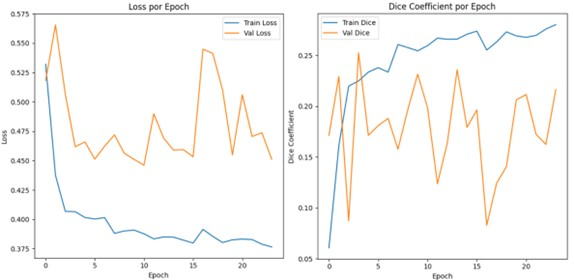
\includegraphics[width=\textwidth]{figures/Figure 1.jpg}
    \caption{Training and validation loss curves for the 3D U-Net model over 24 epochs. The training loss (blue) decreases steadily, while the validation Dice coefficient (orange) improves and stabilizes around epoch 20, indicating convergence.}
    \label{fig:unet_loss_curve}
\end{figure}

\begin{table}[tp]
\centering
\begin{tabular}{lc}
\toprule
\textbf{Metric} & \textbf{Mean ± SD} \\
\midrule
Dice & $0.294 \pm 0.282$ \\
IoU & $0.207 \pm 0.221$ \\
\bottomrule
\end{tabular}
\caption{Performance Metrics: 3D U-Net on the Test Set (N=25). The model achieved a mean Dice coefficient of 0.294 and an IoU of 0.207, with considerable variability across cases, as indicated by the standard deviation.}
\label{tab:unet_metrics}
\end{table}

Qualitative examples of the model outputs are presented in Figure \ref{fig:unet_qualitative}, showing the ground truth in green and predicted segmentation masks in red, in both 2D slices and 3D reconstructions for representative test cases. Figure \ref{fig:unet_qualitative} illustrates the best-performing case, with a Dice coefficient of 0.811, and an intermediate case, with a Dice of 0.342, highlighting the variability in segmentation accuracy across the dataset.

\begin{figure}[tp]
    \centering
    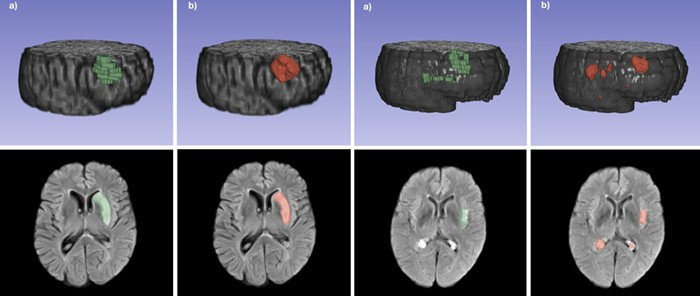
\includegraphics[width=\textwidth]{figures/Figure 2.jpg}
    \caption{Qualitative Results: 3D U-Net Segmentations. The middle-left side shows the best-performing test case (Dice = 0.811), while the middle-right side presents an intermediate case (Dice = 0.342). Each case includes axial, sagittal, and coronal views of the FLAIR image with overlaid ground truth (green) and predicted segmentation (red), as well as a 3D rendering of the lesion. The model accurately captures lesion boundaries in the best case but struggles with diffuse regions in the intermediate case.}
    \label{fig:unet_qualitative}
\end{figure}


\subsection{nnU-Net Results} \label{subsec:nnu-net}  

The nnU-Net model was trained for 141 epochs, with training and validation loss curves shown in Figure \ref{fig:nnu-net_loss_curve}. The validation Dice coefficient improved consistently, stabilizing around epoch 120. Test set results are summarized in Table \ref{tab:nnunet_metrics}.

\begin{figure}[tp]
    \centering
    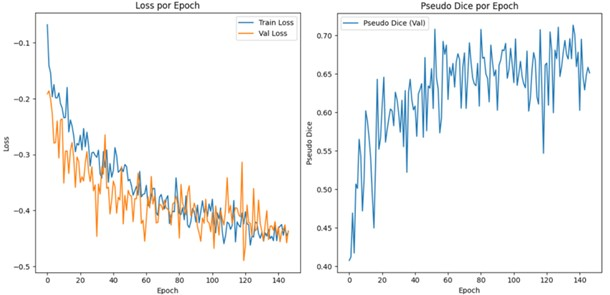
\includegraphics[width=\textwidth]{figures/Figure 3.jpg}
    \caption{Training and validation loss curves for the nnU-Net model over 141 epochs. The training loss (blue) decreases steadily, while the validation Dice coefficient (orange) improves and stabilizes around epoch 120, indicating convergence.}
    \label{fig:nnu-net_loss_curve}
\end{figure}

\begin{table}[tp]
\centering
\begin{tabular}{lc}
\toprule
\textbf{Metric} & \textbf{Mean ± SD} \\
\midrule
Dice & $0.483 \pm 0.284$ \\
IoU & $0.362 \pm 0.244$ \\
\bottomrule
\end{tabular}
\caption{Performance Metrics: nnU-Net on the Test Set (N=25). The model achieved a mean Dice coefficient of 0.483 and an IoU of 0.362, demonstrating improved accuracy and robustness compared to the classical U-Net.}
\label{tab:nnunet_metrics}
\end{table}

The nnU-Net model automatically configured its preprocessing, patch size, and training schedule. It reached optimal validation performance after 141 epochs, as indicated by the decreasing loss curve and the rise of the pseudo-Dice score, showed in Figure \ref{fig:nnu-net_loss_curve}. The average results on the test set are displayed in Table \ref{tab:nnunet_metrics}.

Visual results demonstrated that nnU-Net effectively captured lesion boundaries and spatial continuity, even in cases with irregular shapes or heterogeneous intensities. Figure \ref{fig:nnunet_qualitative} illustrates representative segmentations for two test cases (Dice 0.824 and 0.480), showing good agreement between the predicted and manual annotations.

\begin{figure}[tp]    
    \centering
    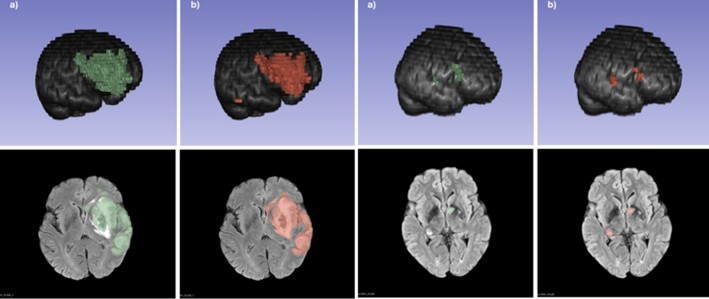
\includegraphics[width=\textwidth]{figures/Figure 4.jpg}
    \caption{Qualitative Results: nnU-Net Segmentations. The left side shows a high-performing test case (Dice = 0.824), while the right side presents a moderate case (Dice = 0.480). Each case includes axial, sagittal, and coronal views of the FLAIR image with overlaid ground truth (green) and predicted segmentation (red), as well as a 3D rendering of the lesion. The model accurately captures lesion boundaries in both cases, demonstrating its robustness across varying lesion characteristics.}
    \label{fig:nnunet_qualitative}
\end{figure}


\subsection{YOLOv8 Results} \label{subsec:yolov8}

The YOLOv8-seg model was trained for 100 epochs, with training and validation loss curves shown in Figure \ref{fig:yolov8_loss_curve}. The model achieved a mean Average Precision (mAP) of 0.512 on the validation set. Test set results, including Dice coefficient, IoU, precision, and recall, are summarized in Table \ref{tab:yolov8_metrics} and Table \ref{tab:yolov8_detection_metrics}.

\begin{figure}[tp]
    \centering
    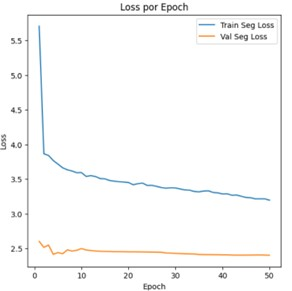
\includegraphics[width=.7\textwidth]{figures/Figure 5.jpg}
    \caption{Training and validation loss curves for the YOLOv8-seg model over 100 epochs. The training loss (blue) decreases rapidly, while the validation Dice coefficient (orange) improves and stabilizes around epoch 50, indicating convergence.}
    \label{fig:yolov8_loss_curve}
\end{figure}

\begin{table}[tp]
\centering
\begin{tabular}{lc}
\toprule
\textbf{Metric} & \textbf{Mean ± SD} \\
\midrule
Dice & $0.476 \pm 0.287$ \\
IoU & $0.358 \pm 0.254$ \\
\bottomrule
\end{tabular}
\caption{Performance Metrics: YOLOv8-seg on the Test Set (N=25). The model achieved a mean Dice coefficient of 0.476 and an IoU of 0.358, demonstrating competitive performance with efficient inference capabilities.}
\label{tab:yolov8_metrics}
\end{table}

\begin{table}[tp]
\centering
\begin{tabular}{lc}
\toprule
\textbf{Metric} & \textbf{Mean ± SD} \\
\midrule
Precision & $0.437 \pm 0.057$ \\
Recall & $0.213 \pm 0.031$ \\
mAP@0.5 & $0.202 \pm 0.034$ \\
mAP@0.5:0.95 & $0.073 \pm 0.014$ \\
\bottomrule
\end{tabular}
\caption{Performance Metrics: YOLOv8 on the Test Set (N=25). The model achieved a mean Average Precision (mAP) of 0.202 at IoU threshold 0.5 and 0.073 at IoU thresholds from 0.5 to 0.95, indicating its effectiveness in detecting ischemic lesions with reasonable precision and recall.}
\label{tab:yolov8_detection_metrics}
\end{table}

The YOLOv8 segmentation variant was trained on 2D FLAIR slices reconstructed into 3D volumes for evaluation. The loss curve showed rapid convergence after 50 epochs as is shown in Figure \ref{fig:yolov8_loss_curve}. Quantitative metrics for validation are summarized in Table \ref{tab:yolov8_metrics}, while the final test results are presented in Table \ref{tab:comparison}.

Qualitatively, YOLOv8 achieved fast inference and detected most lesion regions, as shown in Figure \ref{fig:yolov8_qualitative}, but its segmentations tended to be slightly less precise than those of the 3D networks, occasionally missing fine structures or small peripheral lesions.

\begin{figure}[tp]
    \centering
    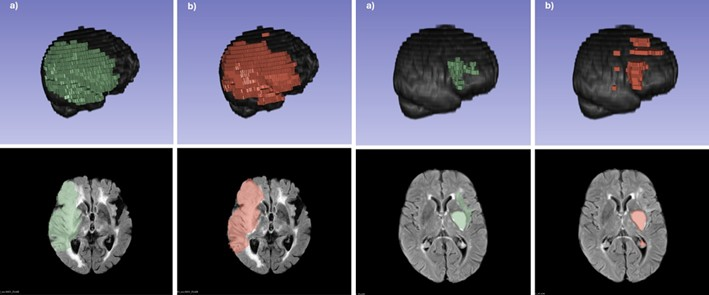
\includegraphics[width=\textwidth]{figures/Figure 6.jpg}
    \caption{Qualitative Results: YOLOv8 Segmentations. The left side shows a high-performing test case (Dice = 0.792), while the right side presents a moderate case (Dice = 0.365). Each case includes axial, sagittal, and coronal views of the FLAIR image with overlaid ground truth (green) and predicted segmentation (red), as well as a 3D rendering of the lesion. The model captures major lesion areas but may miss finer details compared to 3D models.}
    \label{fig:yolov8_qualitative}
\end{figure}


\subsection{Summarized Results Comparison} \label{subsec:comparison}

A comparative overview of the three architectures is provided in Table \ref{tab:comparison}. As shown in Table \ref{tab:comparison}, nnU-Net achieved the highest Dice and IoU values across all patient cases, followed by YOLOv8 and U-Net. These quantitative findings confirm the influence of model design and dimensionality on segmentation accuracy.

\begin{table}[h]
\centering
\begin{tabular}{lccc}
\toprule
\textbf{Model} & \textbf{Dice} & \textbf{IoU} & \textbf{Notes} \\
\midrule
U-Net & $0.294 \pm 0.282$ & $0.207 \pm 0.221$ & Stable training; limited generalization to complex lesions \\
nnU-Net & $0.483 \pm 0.284$ & $0.362 \pm 0.244$ & Best overall performance and most consistent segmentation \\
YOLOv8 & $0.476 \pm 0.287$ & $0.358 \pm 0.254$ & Fastest inference; lower boundary accuracy \\
\bottomrule
\end{tabular}
\caption{Comparison of Segmentation Models on the Test Set (N=25). The nnU-Net achieved the highest Dice and IoU scores, indicating superior segmentation accuracy and robustness. YOLOv8 provided competitive performance with efficient inference, while U-Net showed limited generalization capabilities.}
\label{tab:comparison}
\end{table}

\section{Discussion} \label{sec:discussion}

%This section discusses the comparative performance of the three segmentation models, highlighting their strengths and limitations, as well as potential clinical implications and future research directions.

The comparative analysis highlights distinct characteristics in the performance of U-Net, nnU-Net, and YOLOv8 for ischemic lesion segmentation in FLAIR MRI images.

The U-Net architecture achieved moderate performance across the validation and test sets. Despite its well-established effectiveness in biomedical image segmentation, the model exhibited considerable variability among individual cases. Quantitatively, the Dice and IoU metrics indicated that the network was capable of correctly identifying lesions in certain cases but failed to generalize consistently across the dataset. This uneven behavior suggests that the classical U-Net is highly sensitive to image quality and lesion contrast. In cases where boundaries were well defined, segmentation was accurate, while diffuse or low-contrast lesions often led to missed detections.

The relatively high standard deviation observed in the test results indicates limited robustness. This variability may stem from the restricted size of the dataset and from the intrinsic heterogeneity of ischemic lesions. Additionally, the classic U-Net requires extensive manual configuration, including input size definition, normalization strategy, and data augmentation parameters. These manual design choices can introduce performance fluctuations depending on how well they adapt to the dataset characteristics.

The nnU-Net outperformed the classical U-Net in both validation and test phases. Its self-configuring mechanism automatically selected preprocessing, normalization, and training hyperparameters, leading to higher Dice and IoU scores. The model demonstrated a strong ability to adapt to the dataset and segment complex or irregular lesions, confirming the effectiveness of automated optimization. However, some test cases still produced null segmentations, revealing that even advanced configurations can struggle with highly heterogeneous or low-quality images.

The improved consistency observed in nnU-Net reflects its capacity to generalize better from limited data. Nevertheless, the standard deviation across test results indicates residual instability, possibly due to the reduced number of samples and to contrast variations between scans. In addition, nnU-Net is computationally demanding, requiring long training times and significant GPU resources, which may limit its practical deployment in resource-constrained environments.

Although originally designed for object detection rather than medical segmentation, YOLOv8 achieved competitive results in this study. Its inference speed and implementation simplicity stand out as major advantages, making it suitable for real-time applications. The model achieved respectable Dice and IoU values, occasionally matching those of nnU-Net in favorable cases. However, it also exhibited variability, with some test cases showing incomplete or missing lesion predictions.

This behavior can be explained by YOLOv8’s design, which prioritizes detection speed and bounding-box optimization over pixel-level precision. Consequently, the model performs well when lesions are clearly delimited but tends to underestimate diffuse or low-contrast regions. Despite these limitations, YOLOv8 demonstrates strong potential for fast and flexible segmentation pipelines, especially if adapted with domain-specific augmentations or loss functions.

When comparing all three architectures, nnU-Net achieved the highest accuracy and stability, confirming the benefits of automatic configuration in medical image segmentation. U-Net, while less resource-intensive, showed limited generalization, particularly in challenging cases. YOLOv8, though less precise, offered the best balance between speed and usability. These results emphasize that performance depends not only on network complexity but also on the suitability of the architecture to the dataset characteristics. 

However, several limitations must be acknowledged. The study was conducted on a relatively small dataset of 250 cases, using only FLAIR sequences, which restricts the models’ ability to exploit complementary multimodal information (e.g., DWI or ADC). Computational constraints limited full cross-validation in nnU-Net and reduced hyperparameter optimization in the other models. Moreover, the evaluation focused exclusively on segmentation accuracy without assessing the real clinical impact.

Future research could focus on incorporating multimodal MRI sequences (e.g., DWI and ADC) to improve lesion characterization and model generalization. In addition to classical data augmentation techniques, the creation of larger and more diverse datasets through the inclusion of new clinical cases and the integration of complementary public databases would be essential to achieve greater robustness. From a methodological perspective, combining 3D segmentation architectures with lightweight 2D frameworks like YOLOv8 could lead to hybrid models that preserve spatial precision while maintaining high computational efficiency. Such developments would contribute to the design of reliable and time-efficient automated systems for early ischemic stroke screening and diagnosis.

\section{Conclusion} \label{sec:conclusion}

%This study presented a comparative analysis of three deep learning architectures—U-Net, nnU-Net, and YOLOv8—for the segmentation of ischemic stroke lesions in FLAIR MRI images. Each model demonstrated unique strengths and limitations, influenced by their design philosophies and adaptability to the dataset characteristics.

This study presented a comparative analysis of three deep learning architectures—U-Net, nnU-Net, and YOLOv8—for the automatic segmentation of ischemic stroke lesions in FLAIR MRI images. The main objective was to evaluate their performance, analyze their respective strengths and weaknesses, and assess their feasibility for clinical use. The results demonstrate that deep learning techniques can achieve accurate and reproducible segmentation of ischemic lesions even without the use of contrast-enhanced imaging, supporting the potential of artificial intelligence for early stroke detection and screening.

The experimental findings show that nnU-Net achieved the highest overall accuracy, obtaining the best Dice and IoU scores and exhibiting strong generalization across cases. Its self-configuring design proved particularly effective in adapting the model to the dataset characteristics, minimizing the need for manual tuning. U-Net, despite its widespread use as a baseline in biomedical segmentation, achieved the lowest performance among the evaluated models. Its results were less accurate and more variable, confirming the limitations of manually configured architectures when applied to heterogeneous clinical data. YOLOv8, originally designed for object detection, offered competitive performance and the fastest inference time, highlighting its potential for real-time or resource-constrained applications.

These outcomes indicate that no single architecture dominates in all aspects; rather, each offers complementary advantages. nnU-Net is best suited for research and diagnostic contexts requiring high accuracy, U-Net serves as a methodological baseline that provides a reference for evaluating more advanced models, and YOLOv8 enables rapid deployment in clinical workflows where processing speed is crucial. Together, they demonstrate that automated segmentation of ischemic lesions is technically feasible and can be integrated into radiological pipelines to support decision-making and reduce manual workload.

The achievement of accurate segmentation without contrast administration has significant implications for non-invasive and cost-efficient stroke assessment. Automated detection can assist radiologists in identifying subtle ischemic regions that might otherwise be overlooked, standardize the diagnostic process, and accelerate treatment planning. These models demonstrate strong potential for real-world implementation as assistive tools within hospital imaging systems or screening platforms. With further validation on larger and more diverse datasets, they could evolve into clinically deployable AI solutions capable of supporting early diagnosis, personalized monitoring, and potentially near real-time MRI analysis in emergency settings.

In conclusion, this work confirms that deep learning-based segmentation provides a promising pathway toward automated, precise, and accessible tools for ischemic stroke detection. By combining accuracy, adaptability, and computational efficiency, the explored architectures contribute to advancing medical imaging toward faster and more reliable diagnostic support. The integration of such AI-driven solutions into clinical practice could significantly enhance patient care, enabling earlier intervention and better outcomes in one of the world’s leading causes of disability and mortality.

\printbibliography[heading=bibintoc,title={References}]

\end{document}
